\documentclass[a4paper, 12pt]{article}
\usepackage{tikz}
% \usepackage{subfig}
\usepackage{subcaption}
\usetikzlibrary{arrows.meta}
\usepackage{bytefield}
\usepackage[table]{xcolor}
\usepackage{tabularray}
\usepackage{subfig}
% \usepackage[subfigure]{tocloft}
% \usepackage[subfigure]{tocloft}
\usepackage[acronym,xindy]{glossaries}
\UseTblrLibrary{booktabs}

\begin{document}
\begin{titlepage}
  \title{GGAK Format description}
  \author{Júlia M.\\ SatDump \and Aang23\\ SatDump \and Aweeri}
  \maketitle
  \thispagestyle{empty}

  Document describing the format used by Russian satellites that carry GGAK.\par
\end{titlepage}

\cleardoublepage
\pagenumbering{Roman}
\tableofcontents
\cleardoublepage
\addcontentsline{toc}{section}{List of Figures}
\listoffigures
\addcontentsline{toc}{section}{List of Tables}
\listoftables
\cleardoublepage
\newpage

\renewcommand\thepage{\romannumeral\numexpr\value{page}-1\relax}

\pagenumbering{arabic}

\section{Elektro-L 2}

\begin{table}[hb!]
  \centering
  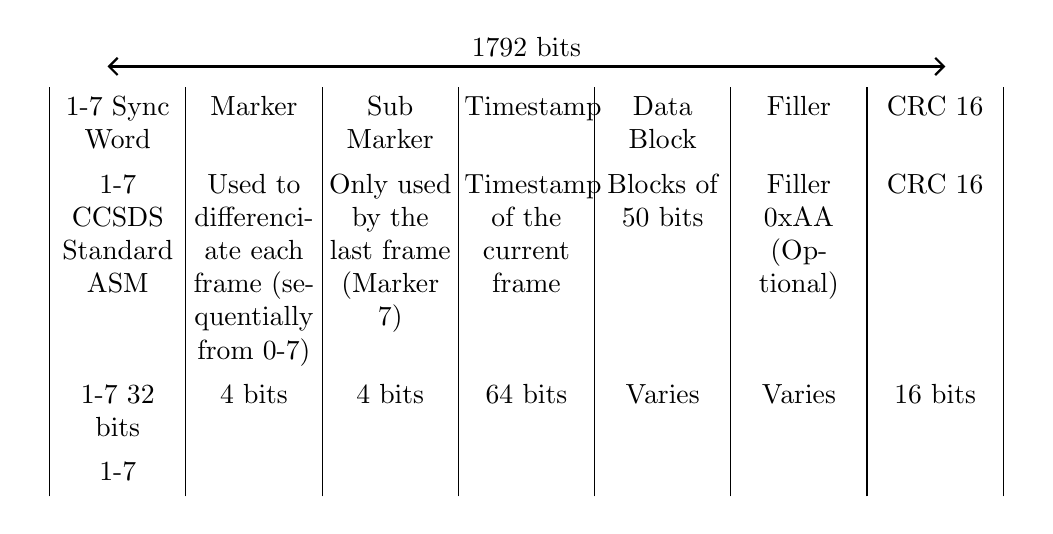
\begin{tikzpicture}
    \node[outer sep=4pt] (m) {
      \begin{tblr}{colsep = 2 pt,
          colspec =
          {|X[0.8,c]|X[0.8,c]|X[0.8,c]|X[0.8,c]|X[0.8,c]|X[0.8,c]|X[0.8,c]|}
        }
        % \SetCell[c=6,r=1]{c}{1792 Bits}\\
        \cmidrule{1-7}
        Sync Word & Marker & Sub Marker & Timestamp & Data Block &
        Filler & CRC 16 \\
        \cmidrule{1-7}
        CCSDS Standard ASM & Used to differenciate each frame
        (sequentially from 0-7) & Only used by the last frame (Marker 7)
        & Timestamp of the current frame & Blocks of 50 bits & Filler
        0xAA (Optional) & CRC 16 \\
        \cmidrule{1-7}
        32 bits & 4 bits & 4 bits & 64 bits & Varies & Varies & 16 bits \\
        \cmidrule{1-7}
      \end{tblr}
    };
    \draw[Straight Barb-Straight Barb, thick, shorten <=10mm, shorten >=10mm]
    (m.north west) -- node[above] {1792 bits}
    (m.north east);
  \end{tikzpicture}
  \label{table:el2}
  \caption{Elektro-L2 GGAK Frame Structure}
\end{table}\par

\begin{figure}[hb!]
  \centering
  % \begin{bytefield}[endianness=little,bitwidth=1.1em\linewitdh]{16}
  \begin{bytefield}[bitheight=4ex,bitwidth=2ex,boxformatting={\centering\small}]{32}
    % \bitheader[endianness=little]{0-31} \\

    \bitheader[endianness=little]{0,7,15,23,31} \\
    % \wordbox{1}{CCSDS Standard ASM} \\ %%% & \bitbox{4}{Marker} &
    % \bitbox{4}{rest} \\
    \bitbox{32}{CCSDS Standard ASM} \\% & \bitboxes{4}{{Marker}{rest}} \\
    \bitboxes{8}{{1A} {CF} {FC} {1D}} \\
    \bitboxes{1}{00011010110011111111110000011101}\\
  \end{bytefield}
  \caption{Elektro-L 2 GGAK - Sync Word}
  \label{fig:eleASM}
\end{figure}

\begin{figure}[hb!]
  \centering
  \captionsetup[subfigure]{labelformat=empty}
  \begin{subfigure}[hb!]{0.5\textwidth}
    \centering
    \begin{bytefield}[bitheight=4ex,bitwidth=4ex,boxformatting={\centering\small}]{8}
      \bitheader[endianness=little]{0,3,4,7} \\
      \bitboxes{4}{{Marker}{Sub Marker}} \\
      \bitboxes{1}{00000000}\\
    \end{bytefield}
    \caption{Marker 0}
  \end{subfigure}%
  \begin{subfigure}[hb!]{0.5\textwidth}
    \centering
    \begin{bytefield}[bitheight=4ex,bitwidth=4ex,boxformatting={\centering\small}]{8}
      \bitheader[endianness=little]{0,3,4,7} \\
      \bitboxes{4}{{Marker}{Sub Marker}} \\
      \bitboxes{1}{00010000}\\
    \end{bytefield}
    \caption{Marker 1}
  \end{subfigure}
  \par\bigskip
  \begin{subfigure}[hb!]{0.5\textwidth}
    \centering
    \begin{bytefield}[bitheight=4ex,bitwidth=4ex,boxformatting={\centering\small}]{8}
      \bitheader[endianness=little]{0,3,4,7} \\
      \bitboxes{4}{{Marker}{Sub Marker}} \\
      \bitboxes{1}{00100000}\\
    \end{bytefield}
    \caption{Marker 2}
  \end{subfigure}%
  \begin{subfigure}[hb!]{0.5\textwidth}
    \centering
    \begin{bytefield}[bitheight=4ex,bitwidth=4ex,boxformatting={\centering\small}]{8}
      \bitheader[endianness=little]{0,3,4,7} \\
      \bitboxes{4}{{Marker}{Sub Marker}} \\
      \bitboxes{1}{00110000}\\
    \end{bytefield}
    \caption{Marker 3}
  \end{subfigure}
  \par\bigskip
  \begin{subfigure}[hb!]{0.5\textwidth}
    \centering
    \begin{bytefield}[bitheight=4ex,bitwidth=4ex,boxformatting={\centering\small}]{8}
      \bitheader[endianness=little]{0,3,4,7} \\
      \bitboxes{4}{{Marker}{Sub Marker}} \\
      \bitboxes{1}{01000000}\\
    \end{bytefield}
    \caption{Marker 4}
  \end{subfigure}%
  \begin{subfigure}[hb!]{0.5\textwidth}
    \centering
    \begin{bytefield}[bitheight=4ex,bitwidth=4ex,boxformatting={\centering\small}]{8}
      \bitheader[endianness=little]{0,3,4,7} \\
      \bitboxes{4}{{Marker}{Sub Marker}} \\
      \bitboxes{1}{01010000}\\
    \end{bytefield}
    \caption{Marker 5}
  \end{subfigure}
  \par\bigskip
  \begin{subfigure}[hb!]{0.5\textwidth}
    \centering
    \begin{bytefield}[bitheight=4ex,bitwidth=4ex,boxformatting={\centering\small}]{8}
      \bitheader[endianness=little]{0,3,4,7} \\
      \bitboxes{4}{{Marker}{Sub Marker}} \\
      \bitboxes{1}{01100000}\\
    \end{bytefield}
    \caption{Marker 6}
  \end{subfigure}
  \par\bigskip
  \begin{subfigure}[hb!]{0.5\textwidth}
    \centering
    \begin{bytefield}[bitheight=4ex,bitwidth=4ex,boxformatting={\centering\small}]{8}
      \bitheader[endianness=little]{0,3,4,7} \\
      \bitboxes{4}{{Marker}{Sub Marker}} \\
      \bitboxes{1}{01110000}\\
    \end{bytefield}
    \caption{Marker 7 - Sub Marker 0}
  \end{subfigure}%
  \begin{subfigure}[hb!]{0.5\textwidth}
    \centering
    \begin{bytefield}[bitheight=4ex,bitwidth=4ex,boxformatting={\centering\small}]{8}
      \bitheader[endianness=little]{0,3,4,7} \\
      \bitboxes{4}{{Marker}{Sub Marker}} \\
      \bitboxes{1}{01110111}\\
    \end{bytefield}
    \caption{Marker 7 - Sub Marker 7}
  \end{subfigure}
  \caption{Elektro-L 2 GGAK - Marker and Sub Marker}
  \label{fig:ele2markers}
\end{figure}

\end{document}
